\documentclass[12pt]{article}
\usepackage{graphicx}
\usepackage{listings}
\usepackage{xcolor}
\definecolor{dkgreen}{rgb}{0,0.6,0}
  \definecolor{gray}{rgb}{0.5,0.5,0.5}
  \definecolor{mauve}{rgb}{0.58,0,0.82}
  \definecolor{greyish}{rgb}{0.96,0.96,0.96}

  \lstset{
    backgroundcolor=\color{greyish},   % choose the background color; you must add \usepackage{color} or \usepackage{xcolor}
    frame=tblr,
    numbers=left,                       % where to put the line-numbers; possible values are (none, left, right)
    numbersep=5pt,                   % how far the line-numbers are from the code
    numberstyle=\tiny\color{mygray}, % the style that is used for the line-numbers
    language=Ruby,
    aboveskip=3mm,
    belowskip=3mm,
    showstringspaces=false,
    columns=flexible,
    basicstyle={\footnotesize\ttfamily},
    numbers=none,
    numberstyle=\tiny\color{gray},
    keywordstyle=\color{blue},
    commentstyle=\color{dkgreen},
    stringstyle=\color{mauve},
    breaklines=true,
    breakatwhitespace=true
    tabsize=1
  }
\begin{document}

\begin{titlepage}
\begin{center} 
 \textsc{\large Facultatea Calculatoare, Informatica si Microelectronica}\\[0.5cm]
\textsc{\large Universitatea Tehnica a Moldovei}\\[1.2cm] 
\vspace{25 mm}

\textsc{\Large Medii Interactive de Dezvoltare a Produselor Soft}\\[0.5cm] 
\textsc{\large Lucrarea de laborator\#4}\\[0.5cm] \newcommand{\HRule}{\rule{\linewidth}{0.5mm}} 
  \vspace{10 mm}
  \HRule \\[0.4cm]
  { \LARGE \bfseries Web development  }\\[0.4cm] 
  \HRule \\[1.5cm]
      \vspace{30mm}

      \begin{minipage}{0.4\textwidth}
      \begin{flushleft} \large
      \emph{Autor:}\\
      Alexandr \textsc{Ialticenco}
      \end{flushleft}
      \end{minipage}
      ~
      \begin{minipage}{0.4\textwidth}
      \begin{flushright} \large
      \emph{lector asistent:} \\
      Irina \textsc{Cojanu} \\ 
      \emph{lector superior:} \\
      Svetlana \textsc{Cojocaru} 
      \end{flushright}
      \end{minipage}\\[4cm]

      \vspace{5 mm}

      \vfill
      \end{center}
      
\end{titlepage}

\section*{Obiectivele lucrarii}
\begin{itemize}
\item Realizarea unui simplu Web Site personal
\item Familiarizarea cu HTML si CSS
\item Interactiuni Javascript
\end{itemize}

\section* {Sarcina lucrarii}
\textbf{Advanced level:}
\begin{itemize}
\item Site-ul trebuie sa contina AJAX Requests.
\item Implimentarea XHR sau JSON responses. Careva din informatie trebuie sa fie dinamic incarcata pe pagina.
\end{itemize}
\section* {Cerinte tehnice}
\begin{itemize}
\item Foloseste MVC (Model–View–Controller) pattern
\end{itemize}
\section {Configurarea Apache + PHP + MySQL}
\subsection{Setarea serverului Apache}
Serverul Apache deja este integrat in sistemul de operare Mac OS X si poate fi usor instalat in alte sisteme de operare.
\newpage 
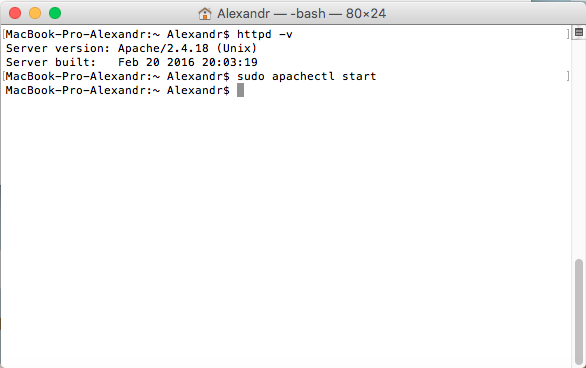
\includegraphics[width=12.5cm]{images/1}
\subsection{Setarea PHP}
Pentru a seta php am decomentat rindul corespunzator in fisierul /etc/apache2/httpd.conf
La fel ca si Apache el este preinstalat in sistemul de operare OS X. Acesta este foarte comod in cazul in care cineva are nevoie de a configura un web server foarte rapid.
\\
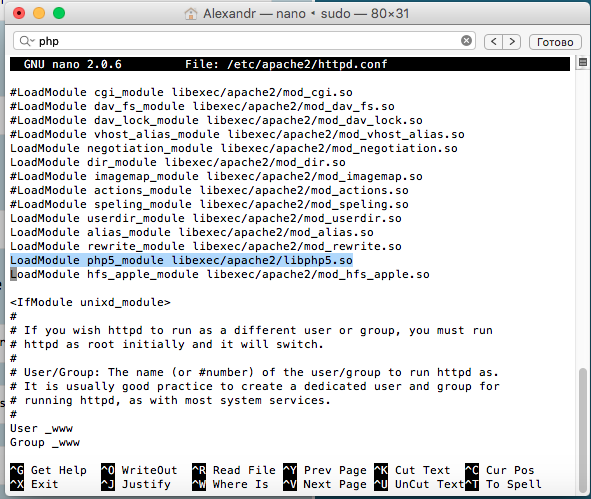
\includegraphics[width=12.5cm]{images/2}
\subsection{Setarea MySQL}
MySQL a fost descarcat de pe site-ul oficial si usor instalat ca un os x package. Pentru comoditate am instalat si configurat phpmyadmin. El este gratuit si foarte simplu in utilizare.\\
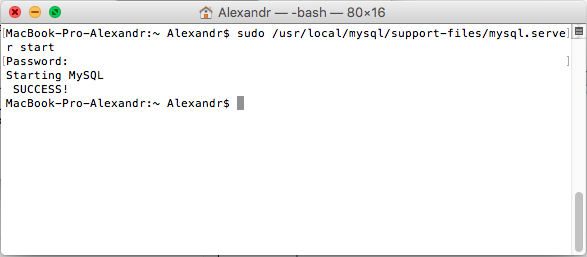
\includegraphics[width=12.5cm]{images/3}\\
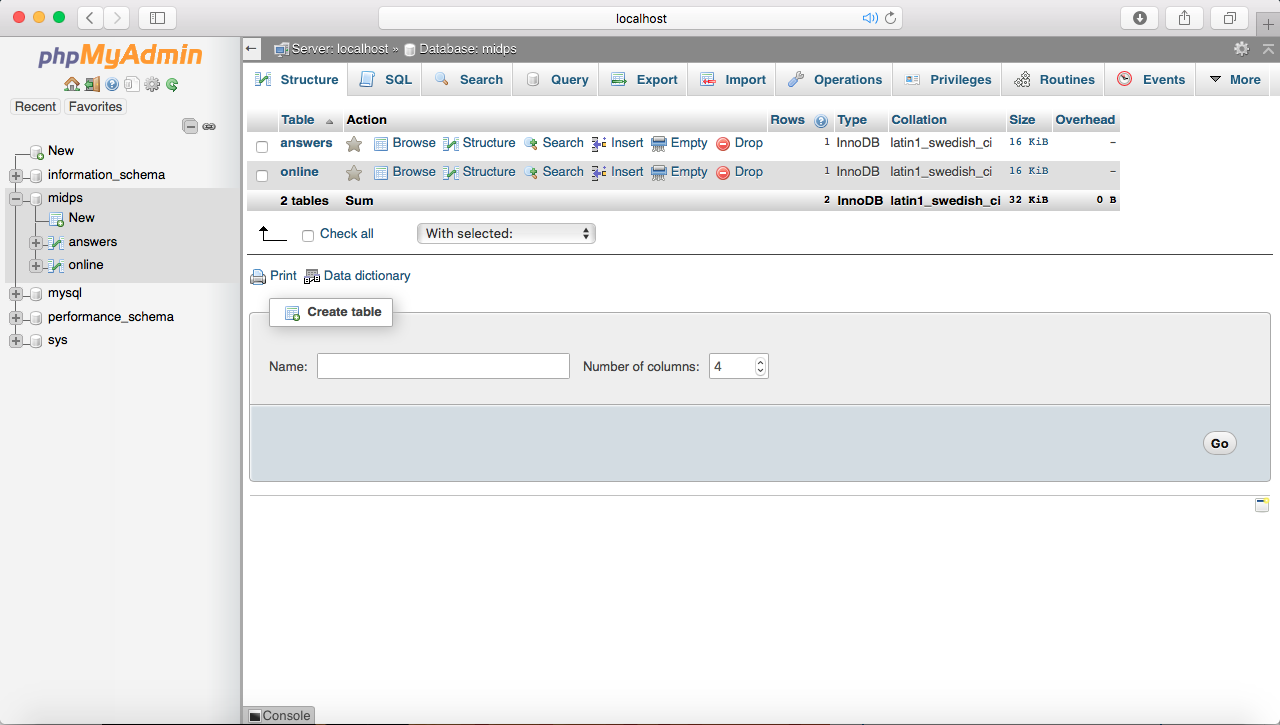
\includegraphics[width=12.5cm]{images/4}
\subsection{Sublime Text}
Ca mediul interactiv de dezvoltare a fost ales Sublime Text, fiindca el este usor, simplu si cu interfata comoda. Mediul dat ofera programatorului Web toate mijloace pentru o munca eficienta. 
\newpage
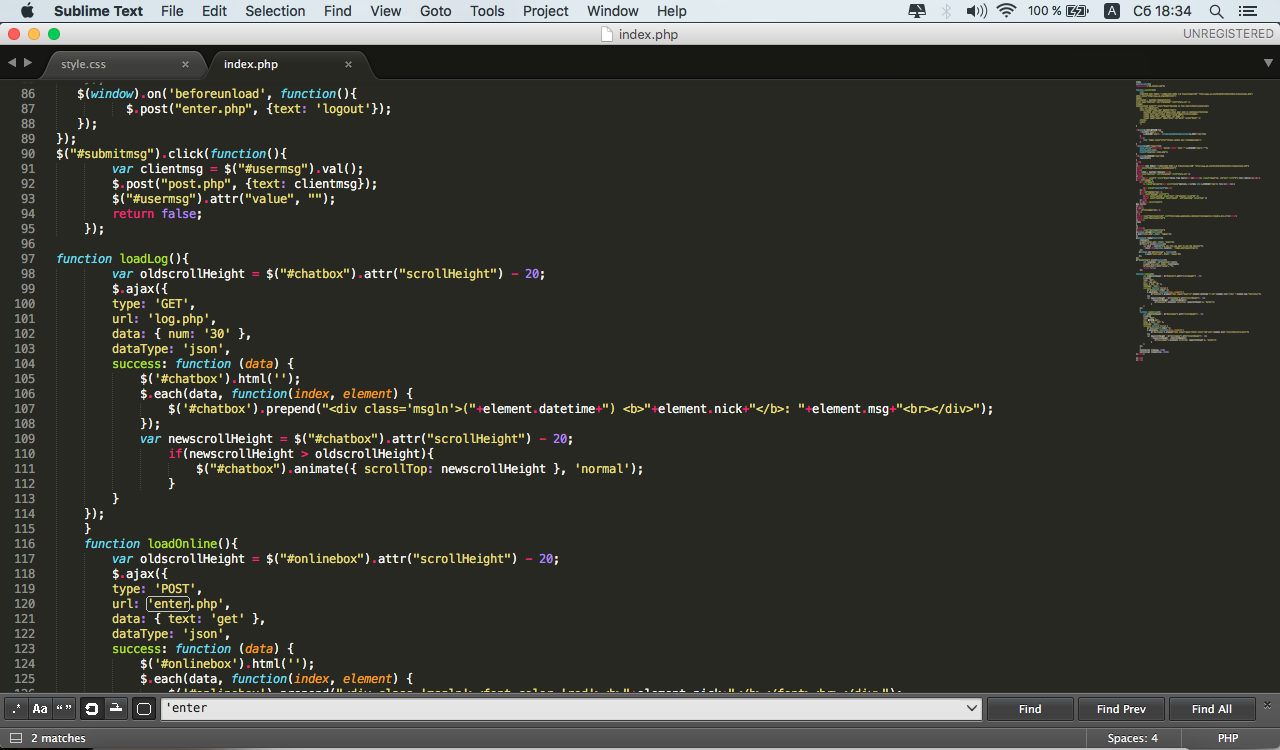
\includegraphics[width=12.5cm]{images/5}
\section {Listingul}
\subsection{Pagina principala}
Pagina index.php reprezinta un mix de html (partial generat de scripturile php) si codul sursa scris in limbajul javascript. Codul php va fi executat de server si nu va fi transmis la client. La inceput serverul verifica, daca este ori nu setat parametru 'name' de sesiunea curenta si daca nu, afiseaza forma de logare. In caz contrar utilizatorul o sa vada chat-ul.
\newpage
\begin{lstlisting}[language=php, caption={Fisierul index.php. Logarea}, label=list2]
<?php
session_start();
require_once("bd_connect.php");
 
function loginForm(){
    echo'
    <!DOCTYPE html PUBLIC "-//W3C//DTD XHTML 1.0 Transitional//EN" "http://www.w3.org/TR/xhtml1/DTD/xhtml1-transitional.dtd">
<html xmlns="http://www.w3.org/1999/xhtml">
<head>
<title>Free Chat</title>
<link type="text/css" rel="stylesheet" href="style.css" />
</head>
<center><font size="5" color="black">Welcome to free Chat!</font></center><br>
    <div id="loginform">
    <form action="index.php" method="post">
        <p><font color="white">Please enter your name to continue:</font></p>
        <label for="name"><font color="white">Name:</font></label>
        <input type="text" name="name" id="name" />
        <input type="submit" name="enter" id="enter" value="Enter" />
    </form>
    </div>
    ';
}
 
if(isset($_POST['enter'])){
    if($_POST['name'] != ""){
        $_SESSION['name'] = stripslashes(htmlspecialchars($_POST['name']));
    }
    else{
        echo '<span class="error">Please select your nickname</span>';
    }
}
if(isset($_GET['logout'])){
    mysql_query("DELETE from `online` WHERE `nick`='".$_SESSION['name']."'");
    session_destroy();
    header("Location: index.php");
}
if(!isset($_SESSION['name'])){
    loginForm();
}	
\end{lstlisting}
Chat-ul reprezinta un simplu div, continutul caruia se modifica prin intermediul jquery (libraria javascript). Scriptul transmite ajax requests, primeste inapoi json-response si-l converteaza in html, care se adauga la html-continutul div-ului chatbox.
\begin{lstlisting}[language=php, caption={Fisierul index.php. Chatbox-ul}, label=list2]
else{
?>
<!DOCTYPE html PUBLIC "-//W3C//DTD XHTML 1.0 Transitional//EN" "http://www.w3.org/TR/xhtml1/DTD/xhtml1-transitional.dtd">
<html xmlns="http://www.w3.org/1999/xhtml">
<head>
<title>Chat - Customer Module</title>
<link type="text/css" rel="stylesheet" href="style.css" />
</head>
<center><font size="5" color="black">Enjoy free Chat!</font></center><p class="logout"><a id="exit" href="#"> (Exit Chat)</a><br><br>
<div id="wrapper">
    <div id="menu">
        <p class="welcome"><font color="white">Welcome, <b><?php echo $_SESSION['name']; ?></b></font></p>

        <div style="clear:both"></div>
    </div>    
    <div id="chatbox"></div>
    <form name="message" action="">
        <input name="usermsg" type="text" id="usermsg" size="63" />
        <input name="submitmsg" type="submit"  id="submitmsg" value="Say" />
    </form>
    <br><font color="white">
Now online:
</font>
<br><br>
<div id="onlinebox"></div>
</div>
<br>
\end{lstlisting}
Acum trebuie sa includem libraria jquery de versiunea 1.7 pentru a face lucru cu javascript mai rapid si simplu
\newpage
\begin{lstlisting}[language=php, caption={Fisierul index.php. Includerea librariei jquery}, label=list2]
<br>
<?php
}
?>
<script type="text/javascript" src="http://ajax.googleapis.com/ajax/libs/jquery/1.7/jquery.min.js">
</script>
\end{lstlisting}
\begin{lstlisting}[language=php, caption={Fisierul index.php. Dezlogarea la inchiderea paginii web}, label=list2]
<script type="text/javascript">
$(window).unload(function(){
$.post("enter.php", {text: 'logout'}); 
}) 
\end{lstlisting}
In cazul logarii sau dezlogarii suntem obligati sa informam scriptul enter.php ca lista de utilizatori online sa fie stocata in baza de date.
\begin{lstlisting}[language=php, caption={Fisierul index.php. On document ready}, label=list2]
$(document).ready(function(){
    loadLog();
    $.post("enter.php", {text: 'login'});  
	$("#exit").click(function(){
		var exit = confirm("Are you sure you want to end the session?");
		if(exit==true){window.location = 'index.php?logout=true';}		
	});
   $(window).on('beforeunload', function(){
          $.post("enter.php", {text: 'logout'}); 
   });
});
\end{lstlisting}
apelam functia loadLog() pentru a initia ajax request care va descarca de pe server ultimele raspunsuri ale utilizatorilor (ca sa nu fie chatbox-ul gol exact dupa logarea). Apoi informam scriptul enter.php ca utilizatorul deja a logat. Mai departe setam link-ul exit ca in cazul apasarii lui sa apara intrebarea daca utilizatorul cu adevarat vrea sa termina sesiunea. La sfarsit setam ca inainte de inchidere a paginii de catre utilizator sa fie informat scriptul enter.php.
\newpage
\begin{lstlisting}[language=php, caption={Fisierul index.php. Trimiterea mesajelor scrise de utilizator}, label=list2]
$("#submitmsg").click(function(){	
		var clientmsg = $("#usermsg").val();
		$.post("post.php", {text: clientmsg});				
		$("#usermsg").attr("value", "");
		return false;
	});
\end{lstlisting}
In cazul apasarii butonului submitmsg prin intermediul post request trimitem mesajul curent scriptului post.php (metoda .post de fapt reprezinta o varianta scurtata a ajax-ului).
\begin{lstlisting}[language=php, caption={Fisierul index.php. metoda loadLog()}, label=list2]
function loadLog(){      
        var oldscrollHeight = $("#chatbox").attr("scrollHeight") - 20;
        $.ajax({ 
        type: 'GET', 
        url: 'log.php', 
        data: { num: '30' }, 
        dataType: 'json',
        success: function (data) { 
            $('#chatbox').html('');
            $.each(data, function(index, element) {
                $('#chatbox').prepend("<div class='msgln'>("+element.datetime+") <b>"+element.nick+"</b>: "+element.msg+"<br></div>");
            });
            var newscrollHeight = $("#chatbox").attr("scrollHeight") - 20;
                if(newscrollHeight > oldscrollHeight){
                    $("#chatbox").animate({ scrollTop: newscrollHeight }, 'normal');
                }               
        }
    });
    }
\end{lstlisting}
Prin intermediul loadLog() descarcam de pe server log-ul mesajelor si le afisam in chatbox. Pentru acesta utilizam ajax http request de tip get cu parametru "num" care contine numarul ultimelor mesaje care vor fi trimise inapoi. Scriptul apelat log.php este setat in asa fel ca sa reintoarca datele in format-ul json. 
\newpage
\begin{lstlisting}[language=php, caption={Fisierul index.php. metoda loadOnline()}, label=list2]
function loadOnline(){      
        var oldscrollHeight = $("#onlinebox").attr("scrollHeight") - 20;
        $.ajax({ 
        type: 'POST', 
        url: 'enter.php', 
        data: { text: 'get' }, 
        dataType: 'json',
        success: function (data) { 
            $('#onlinebox').html('');
            $.each(data, function(index, element) {
                $('#onlinebox').prepend("<div class='msgln'><font color='red'><b>"+element.nick+"</b></font><br></div>");
            });
            var newscrollHeight = $("#onlinebox").attr("scrollHeight") - 20;
                if(newscrollHeight > oldscrollHeight){
                    $("#onlinebox").animate({ scrollTop: newscrollHeight }, 'normal');
                }               
        }
    });
    }\end{lstlisting}
Prin intermediul acestei metode descarcam de pe server lista utilizatorilor care sunt acum ONLINE.
\begin{lstlisting}[language=php, caption={Fisierul index.php. setarea intervalului actualizarii log-ului de mesaje si listei de utilizatori}, label=list2]
	setInterval (loadLog, 500);
    setInterval (loadOnline, 1500);
</script>
</body>
</html>	
\end{lstlisting}

\subsection{Scriptul post.php}
Scriptul post.php primeste ajax-requests de la pagina principala (index.php) si le proceseaza in asa fel ca informatia sa fie stocata in baza de date.
\newpage
\begin{lstlisting}[language=php, caption={Fisierul post.php}, label=list2]
<?
require_once("bd_connect.php");
session_start();
if(isset($_SESSION['name'])){
    mysql_query("INSERT INTO `answers` (`msg`,`stamp`,`datetime`,`nick`) VALUES ('".$_POST['text']."','".time()."','".date("g:i A")."','".$_SESSION['name']."')") or die(mysql_error());
}
?>
\end{lstlisting}
\subsection{Scriptul bd-connect.php}
Scriptul bd-connect.php stabileste conexiunea cu baza de date. El este inclus in alte scripturi ca codul sa nu fie dublat.
\begin{lstlisting}[language=php, caption={Fisierul bd-connect.php}, label=list2]
<?php
header('Content-type: text/html; charset=utf-8');
$db_host = 'localhost';
$db_name = 'midps';
$db_username = 'tester';
$db_password = '12345678';
$connect_to_db = mysql_connect($db_host, $db_username, $db_password) or die("Could not connect: " . mysql_error());
mysql_select_db($db_name, $connect_to_db) or die("Could not select DB: " . mysql_error());
mysql_query("set names utf8");
date_default_timezone_set('Europe/Chisinau');
?>
\end{lstlisting}
\subsection{Scriptul log.php}
Scriptul log.php extrage mesajele scrise de utilizatori din baza de date si le afiseaza in formatul json.
\newpage
\begin{lstlisting}[language=php, caption={Fisierul log.php}, label=list2]
<?php
require_once("bd_connect.php");
$text = $_GET['num'];
$result = mysql_query("SELECT * from `answers`  ORDER BY id DESC LIMIT ".$_GET['num']."") or die(mysql_error());
$return_arr = array();
while ($row = mysql_fetch_array($result)){
	$row_array['msg'] = $row['msg'];
	$row_array['nick'] = $row['nick'];
	$row_array['datetime'] = $row['datetime'];
	array_push($return_arr,$row_array);
}

echo json_encode($return_arr);

?>
\end{lstlisting}
\subsection{Scriptul enter.php}
Scriptul enter.php desfasoara un control asupra logarii si dezlogarii a utilizatorilor in asa fel ca in baza de date (tabelul online) mereu sa fie lista actuala a utilizatorilor online.
	In cazul in care parametru text va fi egal cu login, scriptul va adauga numele utilizatorului la baza de date. In cazul logout - il va sterge. In al treilea caz scriptul va extrage din baza de date lista utilizatorilor logati. Informatiile vor fi puse in json si afisate.
\newpage
\begin{lstlisting}[language=php, caption={Fisierul enter.php}, label=list2]
<?
require_once("bd_connect.php");
session_start();
if(isset($_SESSION['name'])){
    $text = $_POST['text'];
    if ($text == "login")
    mysql_query("INSERT INTO `online` (`nick`) VALUES ('".$_SESSION['name']."')");
else
	if ($text == "logout")
	mysql_query("DELETE from `online` WHERE `nick`='".$_SESSION['name']."'");
else {
	$result = mysql_query("SELECT * from `online`") or die(mysql_error());
$return_arr = array();
while ($row = mysql_fetch_array($result)){
	$row_array['nick'] = $row['nick'];
	array_push($return_arr,$row_array);
}

echo json_encode($return_arr);
}
}
?>\end{lstlisting}
\subsection{Fisierul de marcare style.css}
Proiectul dat utlizeaza un fisier de stil foarte simplu care descrie aparitia chat-ului si alinierea inscriptiilor\newpage
\begin{lstlisting}[language=html, caption={Fisierul style.css}, label=list2]
/* CSS Document */
body {
    font:12px arial;
    color: #222;
    text-align:center;
    padding:35px; }
  
form, p, span {
    margin:0;
    padding:0; }
  
input { font:12px arial; }
  
a {
    color:#0000FF;
    text-decoration:none; }
  
    a:hover { text-decoration:underline; }
  
#wrapper, #loginform {
    margin:0 auto;
    padding-bottom:25px;
    background:#363636;
    width:504px;
    border:1px solid #969696; }
  
#loginform { padding-top:18px; }
  
    #loginform p { margin: 5px; }
  
#chatbox {
    text-align:left;
    margin:0 auto;
    margin-bottom:25px;
    padding:10px;
    background:#fff;
    height:270px;
    width:430px;
    border:1px solid #ACD8F0;
    overflow:auto; }
\end{lstlisting}
\newpage
\begin{lstlisting}[language=html, caption={Fisierul style.css}, label=list2]
#onlinebox {
    text-align:left;
    margin:0 auto;
    margin-bottom:25px;
    padding:10px;
    background:#EBF4FB;
    height:64px;
    width:430px;
    border:1px solid #ACD8F0;
    overflow:auto; }
  
#usermsg {
    width:395px;
    border:1px solid #ACD8F0; }
  
#submit { width: 90px; }
  
.error { color: #ff0000; }
  
#menu { padding:12.5px 25px 12.5px 25px; }
  
.welcome { float:center; }
  
.logout { float:center; }

a {
    color:#ff0000;
}
  
.msgln { margin:0 0 2px 0; }\end{lstlisting}
\section {Folosirea MVC (Model–View–Controller) pattern}
In cadrul acestui proiect ca un model de arhitectura a fost utilizat Model-View-Controller pattern. Astfel utilizatorul actioneaza asupra controalelor (butonul submit, campul de text cu mesajul trimis). Aceste controalele manipuleaza modelul (scripturile post.php, log.php, enter.php), iar modelul in rindul sau actualizeaza View (in cazul nostru div-ul chatbox si div-ul onlinebox). Prin intermediul metodelor loadLog() si loadOnline() componentele arhitecturii de tip View isi schimba continutul (ele sunt subscrise la actualizarile modelei).
\section {Rezultatele}
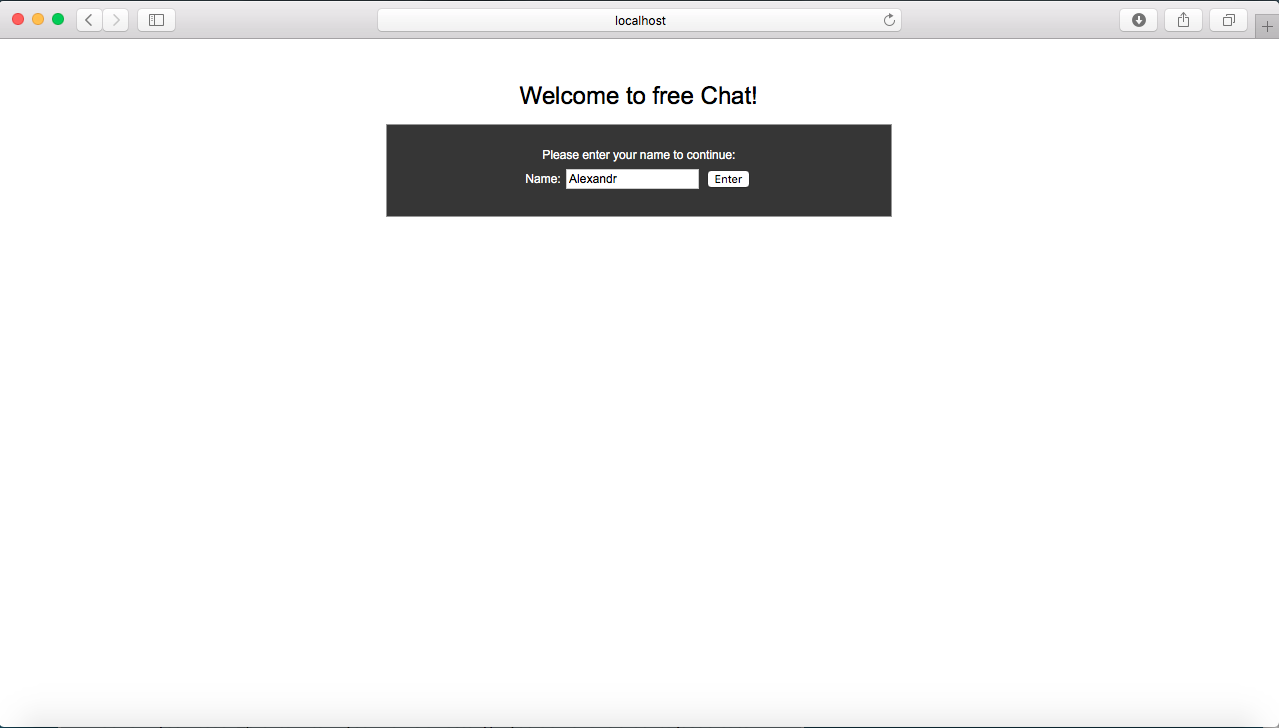
\includegraphics[width=12.5cm]{images/6}\\
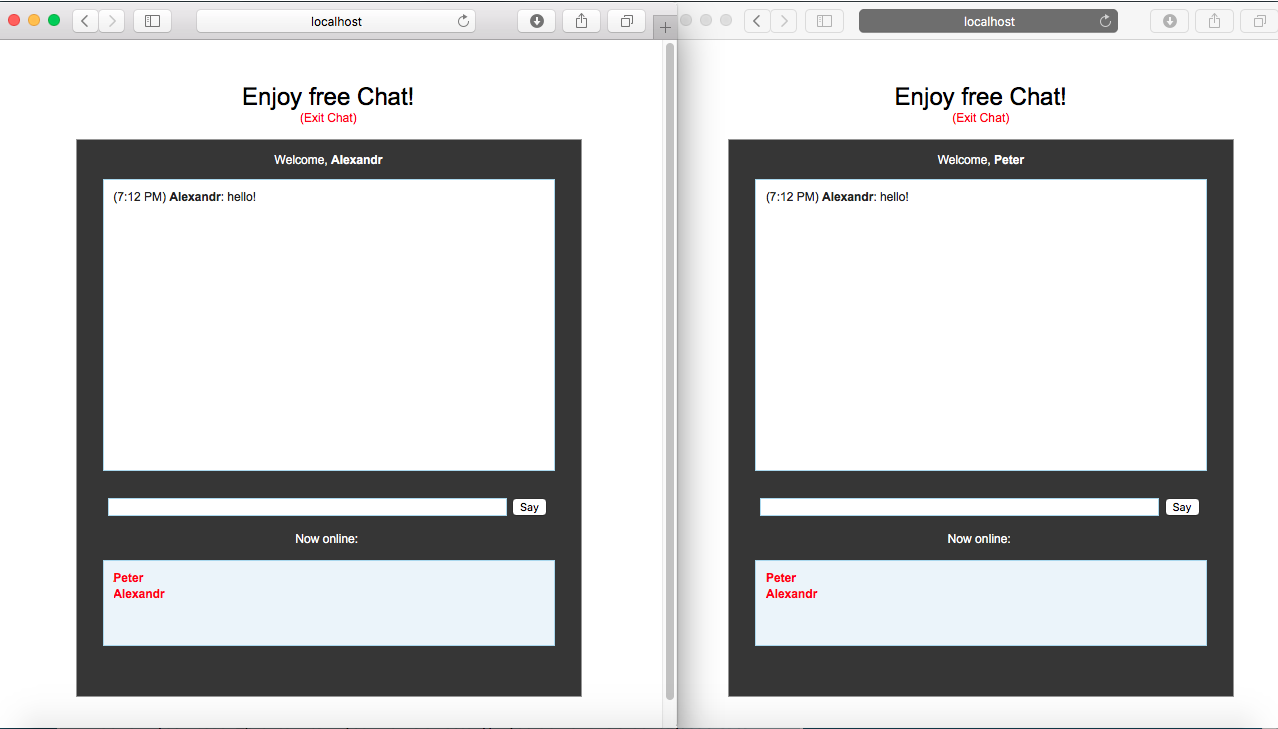
\includegraphics[width=12.5cm]{images/7}\\
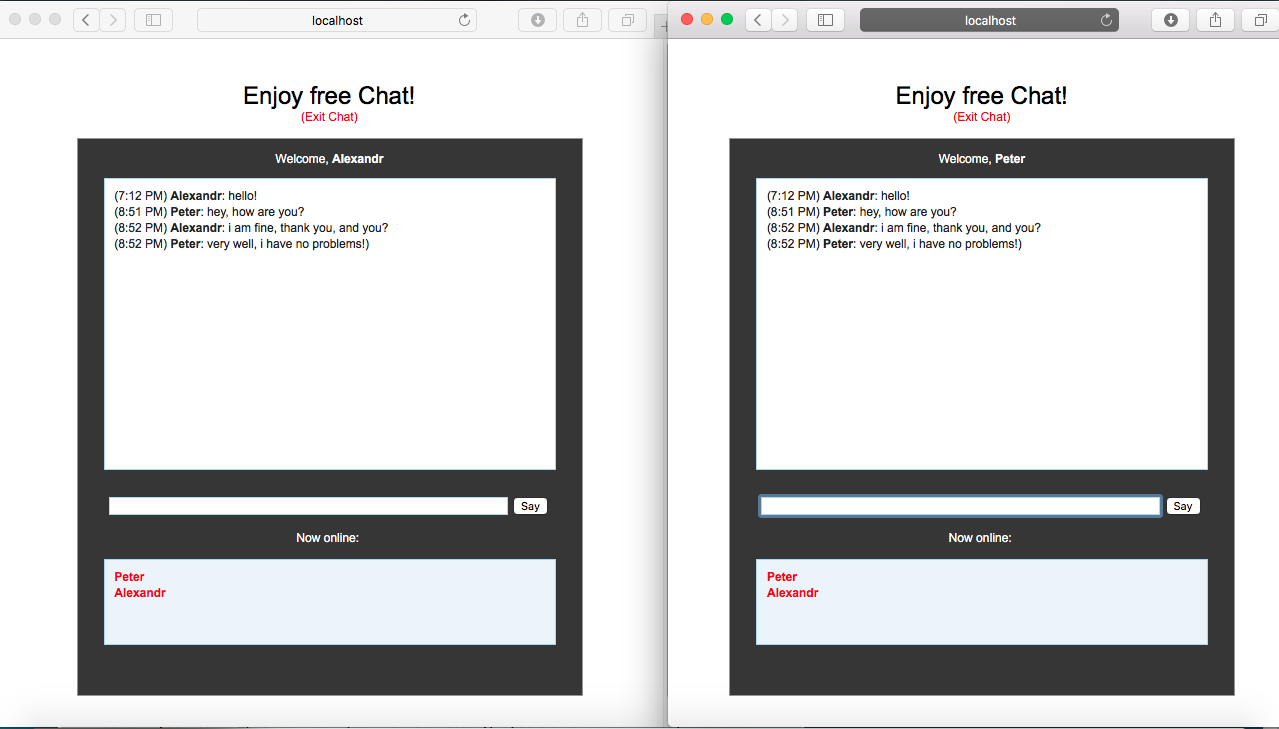
\includegraphics[width=12.5cm]{images/8}
\section*{Concluzii}
In cadrul acestei lucrari de laborator am creat simplu web chat  prin intermediul html, php, javascript si MySQL. Pentru a atinge acest scop am configurat un web-server pe localhost, am invatat arhitectura MVC si am instalat mediul interactiv de dezvoltare Sublime Text.  Cunostintele obtinute pe parcursul desfasurarii lucrarii de laborator vor fi utile pentru realizarea proiectelor ce urmeaza.
\newpage
\section*{Bibliografie}
\begin{enumerate}
\item https://coolestguidesontheplanet.com/get-apache-mysql-php-and-phpmyadmin-working-on-osx-10-11-el-capitan/ - \textbf{Get Apache, MySQL, PHP and phpMyAdmin working on OSX 10.11 El Capitan}
\item https://api.jquery.com - \textbf{JQuery API Documentation}
\item http://php.net/manual/en/ - \textbf{PHP Manual}
\end{enumerate}





\end{document}